\documentclass[12pt, twoside]{article}
\usepackage[letterpaper, margin=1in, headsep=0.5in]{geometry}
\usepackage[english]{babel}
\usepackage[utf8]{inputenc}
\usepackage{amsmath}
\usepackage{amsfonts}
\usepackage{amssymb}
\usepackage{tikz}
\usetikzlibrary{quotes, angles}
\usepackage{graphicx}
\usepackage{enumitem}
\usepackage{multicol}

\newif\ifmeta
\metatrue %print standards and topics tags

\title{Regents Geometry}
\author{Chris Huson}
\date{September 2020}

\usepackage{fancyhdr}
\pagestyle{fancy}
\fancyhf{}
\renewcommand{\headrulewidth}{0pt} % disable the underline of the header
\raggedbottom


\fancyhead[LE]{\thepage}
\fancyhead[RO]{\thepage \\ Name: \hspace{4cm} \,\\}
\fancyhead[LO]{BECA / Dr. Huson / Geometry 10-Trig+similarity+analytics\\* pset ID: 171}

\begin{document}

\subsubsection*{10-6DN-Tangent-situations}
\begin{enumerate}
\item Write down the slope perpendicular to the given slope. \vspace{0.5cm}
  \begin{enumerate}
    \begin{multicols}{2}
    \item   $m= \frac{1}{3} \hspace{1cm} m_{\perp} = $
    \item   $m= -0.8 \hspace{1cm} m_{\perp} = $ 
    \end{multicols}
  \end{enumerate} \vspace{1cm}

\item Write down the center and radius of each circle. Simplify radicals.
  \begin{enumerate}
    \begin{multicols}{2}
    \item   $(x+1)^2+(y+5)^2=49$ \vspace{2cm}
    \item   $(x+1)^2+y^2=50$
    \item   $x^2+4x+y^2-6y=-9$ \vspace{2cm}
    \item   $x^2+y^2-8x=75$
    \end{multicols}
  \end{enumerate}  \vspace{2cm}

  In the following problems, use the point-slope formula: $y-y_1=m (x-x_1)$
\item What is the equation of a line through $(3,-4)$ parallel to the line $y=\frac{3}{2}x-6$?  \vspace{2cm}
\item What is the equation of a line through $(-7,10)$ perpendicular to the line $4x+6y=12$?  \vspace{3cm}
  
\item What is an equation of the perpendicular bisector of $\overline{AB}$ with $A(-2,-7)$ and $B(4,5)$? \vspace{2cm}

\newpage

\item $\triangle ABC$ is shown with $m\angle C=90^\circ$ and the lengths of the triangle's sides are $BC=8$, $AC=15$, and $AB=17$. (not drawn to scale)
  \begin{multicols}{2}
        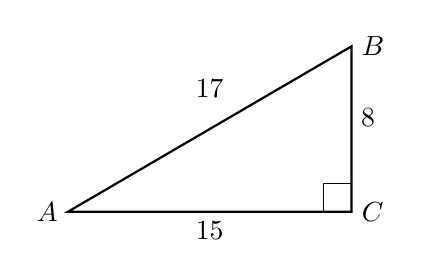
\begin{tikzpicture}[scale=0.6]
          \draw [thick]
          (0,0)node[left]{$A$}--
          (6,0)node[ right]{$C$}--
          (6,3.5)node[right]{$B$}--cycle;
          \draw (6,0)++(-0.6,0)--++(0,0.6)--+(0.6,0);
          \node at (3,0)[below]{$15$};
          \node at (6,2)[right]{$8$};
          \node at (3,2.2)[above]{$17$};
        \end{tikzpicture}
        \begin{enumerate}
        \item Write down the value of $\tan A$. \vspace{0.5cm}
        \item Find the measure of $\angle A$.  \vspace{1cm}
      \end{enumerate}
    \end{multicols} \vspace{2cm}

\item The following diagram shows a pole BT 1.6 m tall on the roof of a vertical building. \\[0.25cm]
  The angle of elevation of the top of the building from A is  
  $25^\circ$ and the distance from point $A$ to the building is 40 feet. (not drawn to scale)
    \begin{center}
      \begin{tikzpicture}[scale=0.4]
        %\draw [-, thick] (0,0)--(35:23);
        \draw [-, thick] (-4,0)--
        (0,0)--
          (17,0)--
          (22,0)--
          (22,10)--(17,10) node[left]{$B$};
        \draw [-, thick] (17,0)--(17,12)node[left]{$T$};
        \draw [fill] (0,0) circle [radius=0.1] node[below]{$A$};
        \draw [dashed] (0,0)--(17,10);
        \node at (3, 0)[above]{$25^\circ$};
        \node at (-3, 0)[below]{ground};
        \node at (19.5, 5)[above]{building};
      \end{tikzpicture}
      \end{center}
      Find the height of the building to the \emph{nearest foot}.

\end{enumerate}
\end{document}